This section gives an overview of the key components of the solver. The figure \ref{fig_architec} gives an overview 
of the most basic classes and the classes they have ponters to (access to). \\
\begin{figure}[!b]
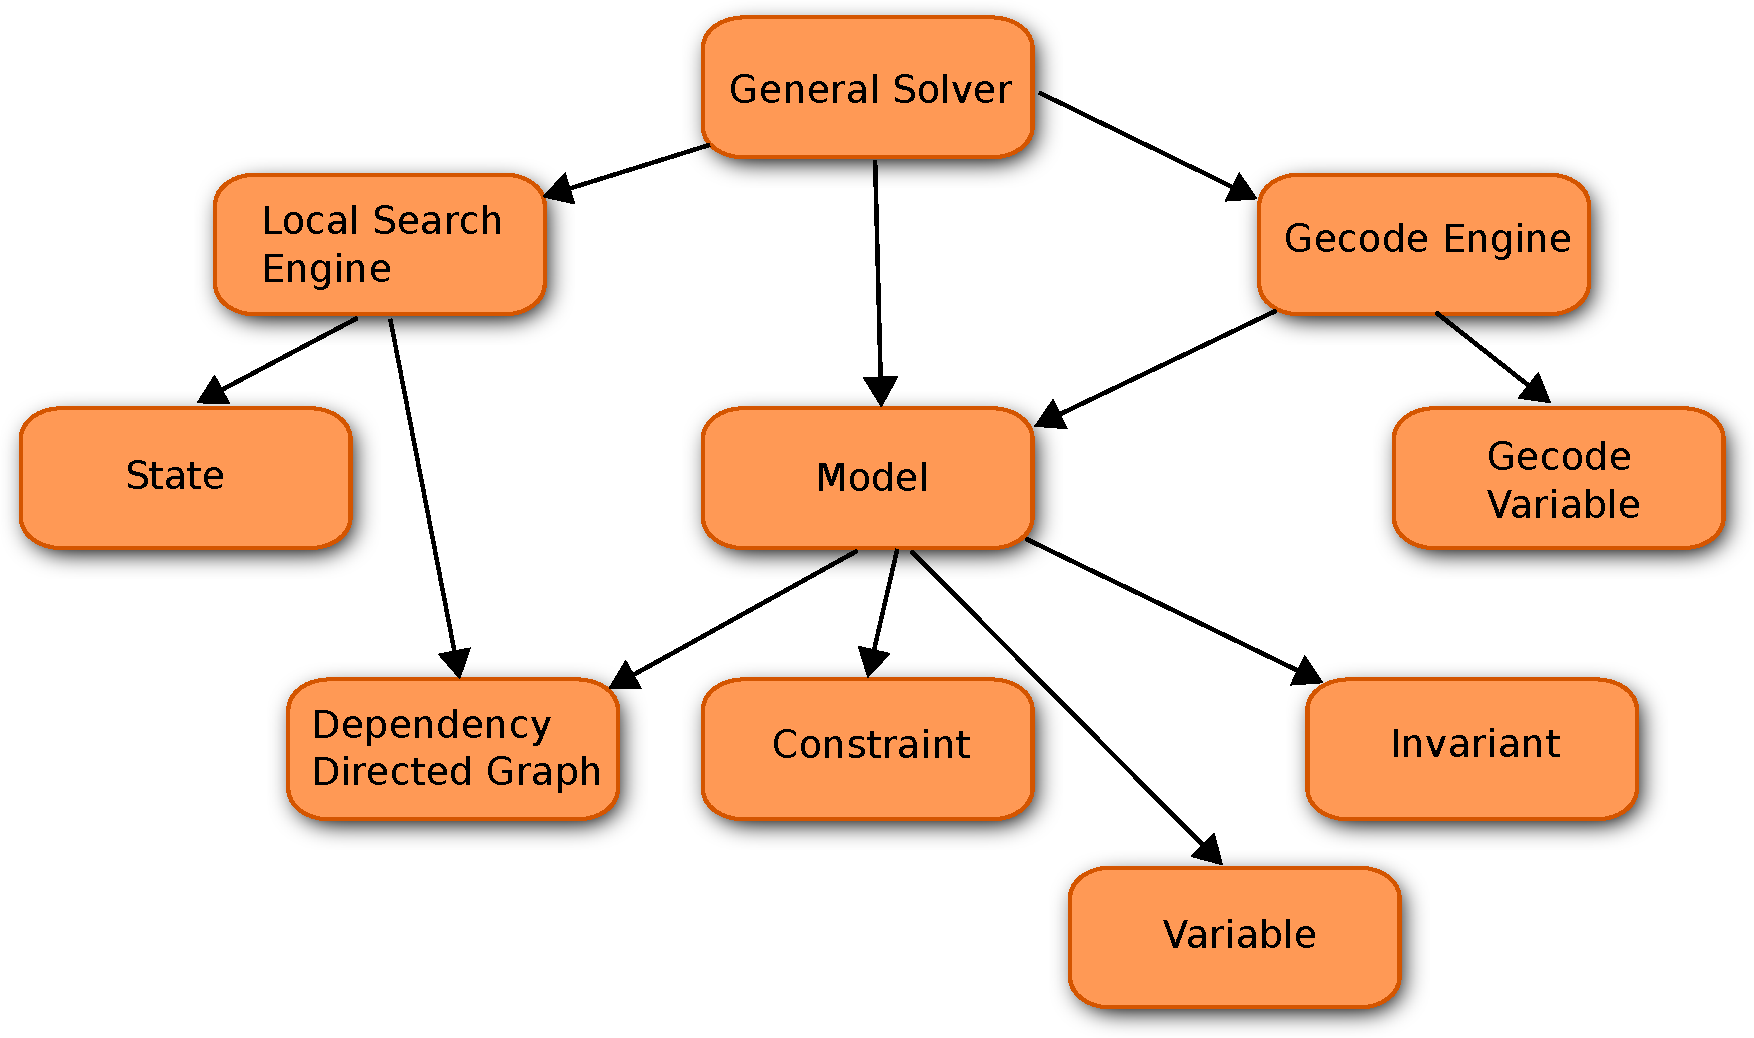
\includegraphics[width=\linewidth]{architectureTest}\caption{Overview of what the classes contains pointers to} 
\label{fig_architec}
\end{figure}
The main part of the solver is the \gensol class that functions like a distribution center, distributing tasks given 
by the user to the right part of the solver. The \gensol class contains 
the methods public to the user, such as creating variables and constraints, finding initial solution and optimizing the 
solution. \\ 
The two engines for solving are the \gecodesol and \lssol that find the initial solution and optimize the solution 
respectively. \gecodesol is used for preprocessing and finding an initial solution if possible with the limits given. 
\boste{Either just timelimit or could be made visible to the user by an option class with node, fail, and time limit.}  
This part will be elaborated further in section \ref{sec_gecode}. \\
\lssol is responsible for the optmization part of the solver with the use of local search and metaheuristics. \lssol 
transform the model to a CBLS model before the local search can start. How this is done and why will be discussed in 
section \ref{sec_ls}. \\ 
The Model class contains all variable, constraints and invariants and is used and altered by the previous three 
classes. Constraint and Invariant are parents to all constraint and invariant classes respectively. The contain 
abstract methods that the child classes must specify. The variable class is the only other class public to the user. A 
variable contains both the variable used by Gecode but is also used for local search. 
